\documentclass[20pt, a0paper, portrait]{tikzposter}

\usepackage[utf8]{inputenc}
\usepackage[T1]{fontenc}
\usepackage{textcomp}
\usepackage{arev}
\usepackage{arevmath}
\usepackage{arevtext}
\usepackage{graphicx}
\usepackage{wrapfig}
\usepackage{microtype}

% Bibliography
\usepackage[backend=biber,
bibencoding=utf8,
bibstyle=numeric-comp,
%style=verbose, %verbose-ibid,
url=true, % include url in reference
doi=true, % include doi in reference
sorting=none, % sorting of citations
%autocite=superscript, % autocite becomes superscript
maxcitenames=1, % Max names displayed when citing in text
maxbibnames=10, % Max number of names displayed in the bibliography
giveninits=true % Use initials
]{biblatex}
\addbibresource{citations.bib}
\renewcommand*{\bibfont}{\footnotesize}

\renewcommand*\familydefault{\sfdefault}

\title{Research}
\author{Engineering Design \& Manufacture Group}
\date{\today}
\institute{University of Bath, UK}

\usetheme{Default}
\usecolorstyle[colorPalette=GreenGrayViolet]{Default}
\useblockstyle{Default}
\usetitlestyle{Filled}
  
\begin{document}

\maketitle

\begin{columns}
  \column{0.5}
  \block[]{RepRap}{
    \textbf{RepRap -- the replicating rapid prototyper}\\
    \small
    R. Jones, P. Haufe, E. Sells, P. Iravani, V. Olliver, C. Palmer \& A. Bowyer\\
    Robotica
    \begin{tikzfigure}[RepRap 3D Printer]
      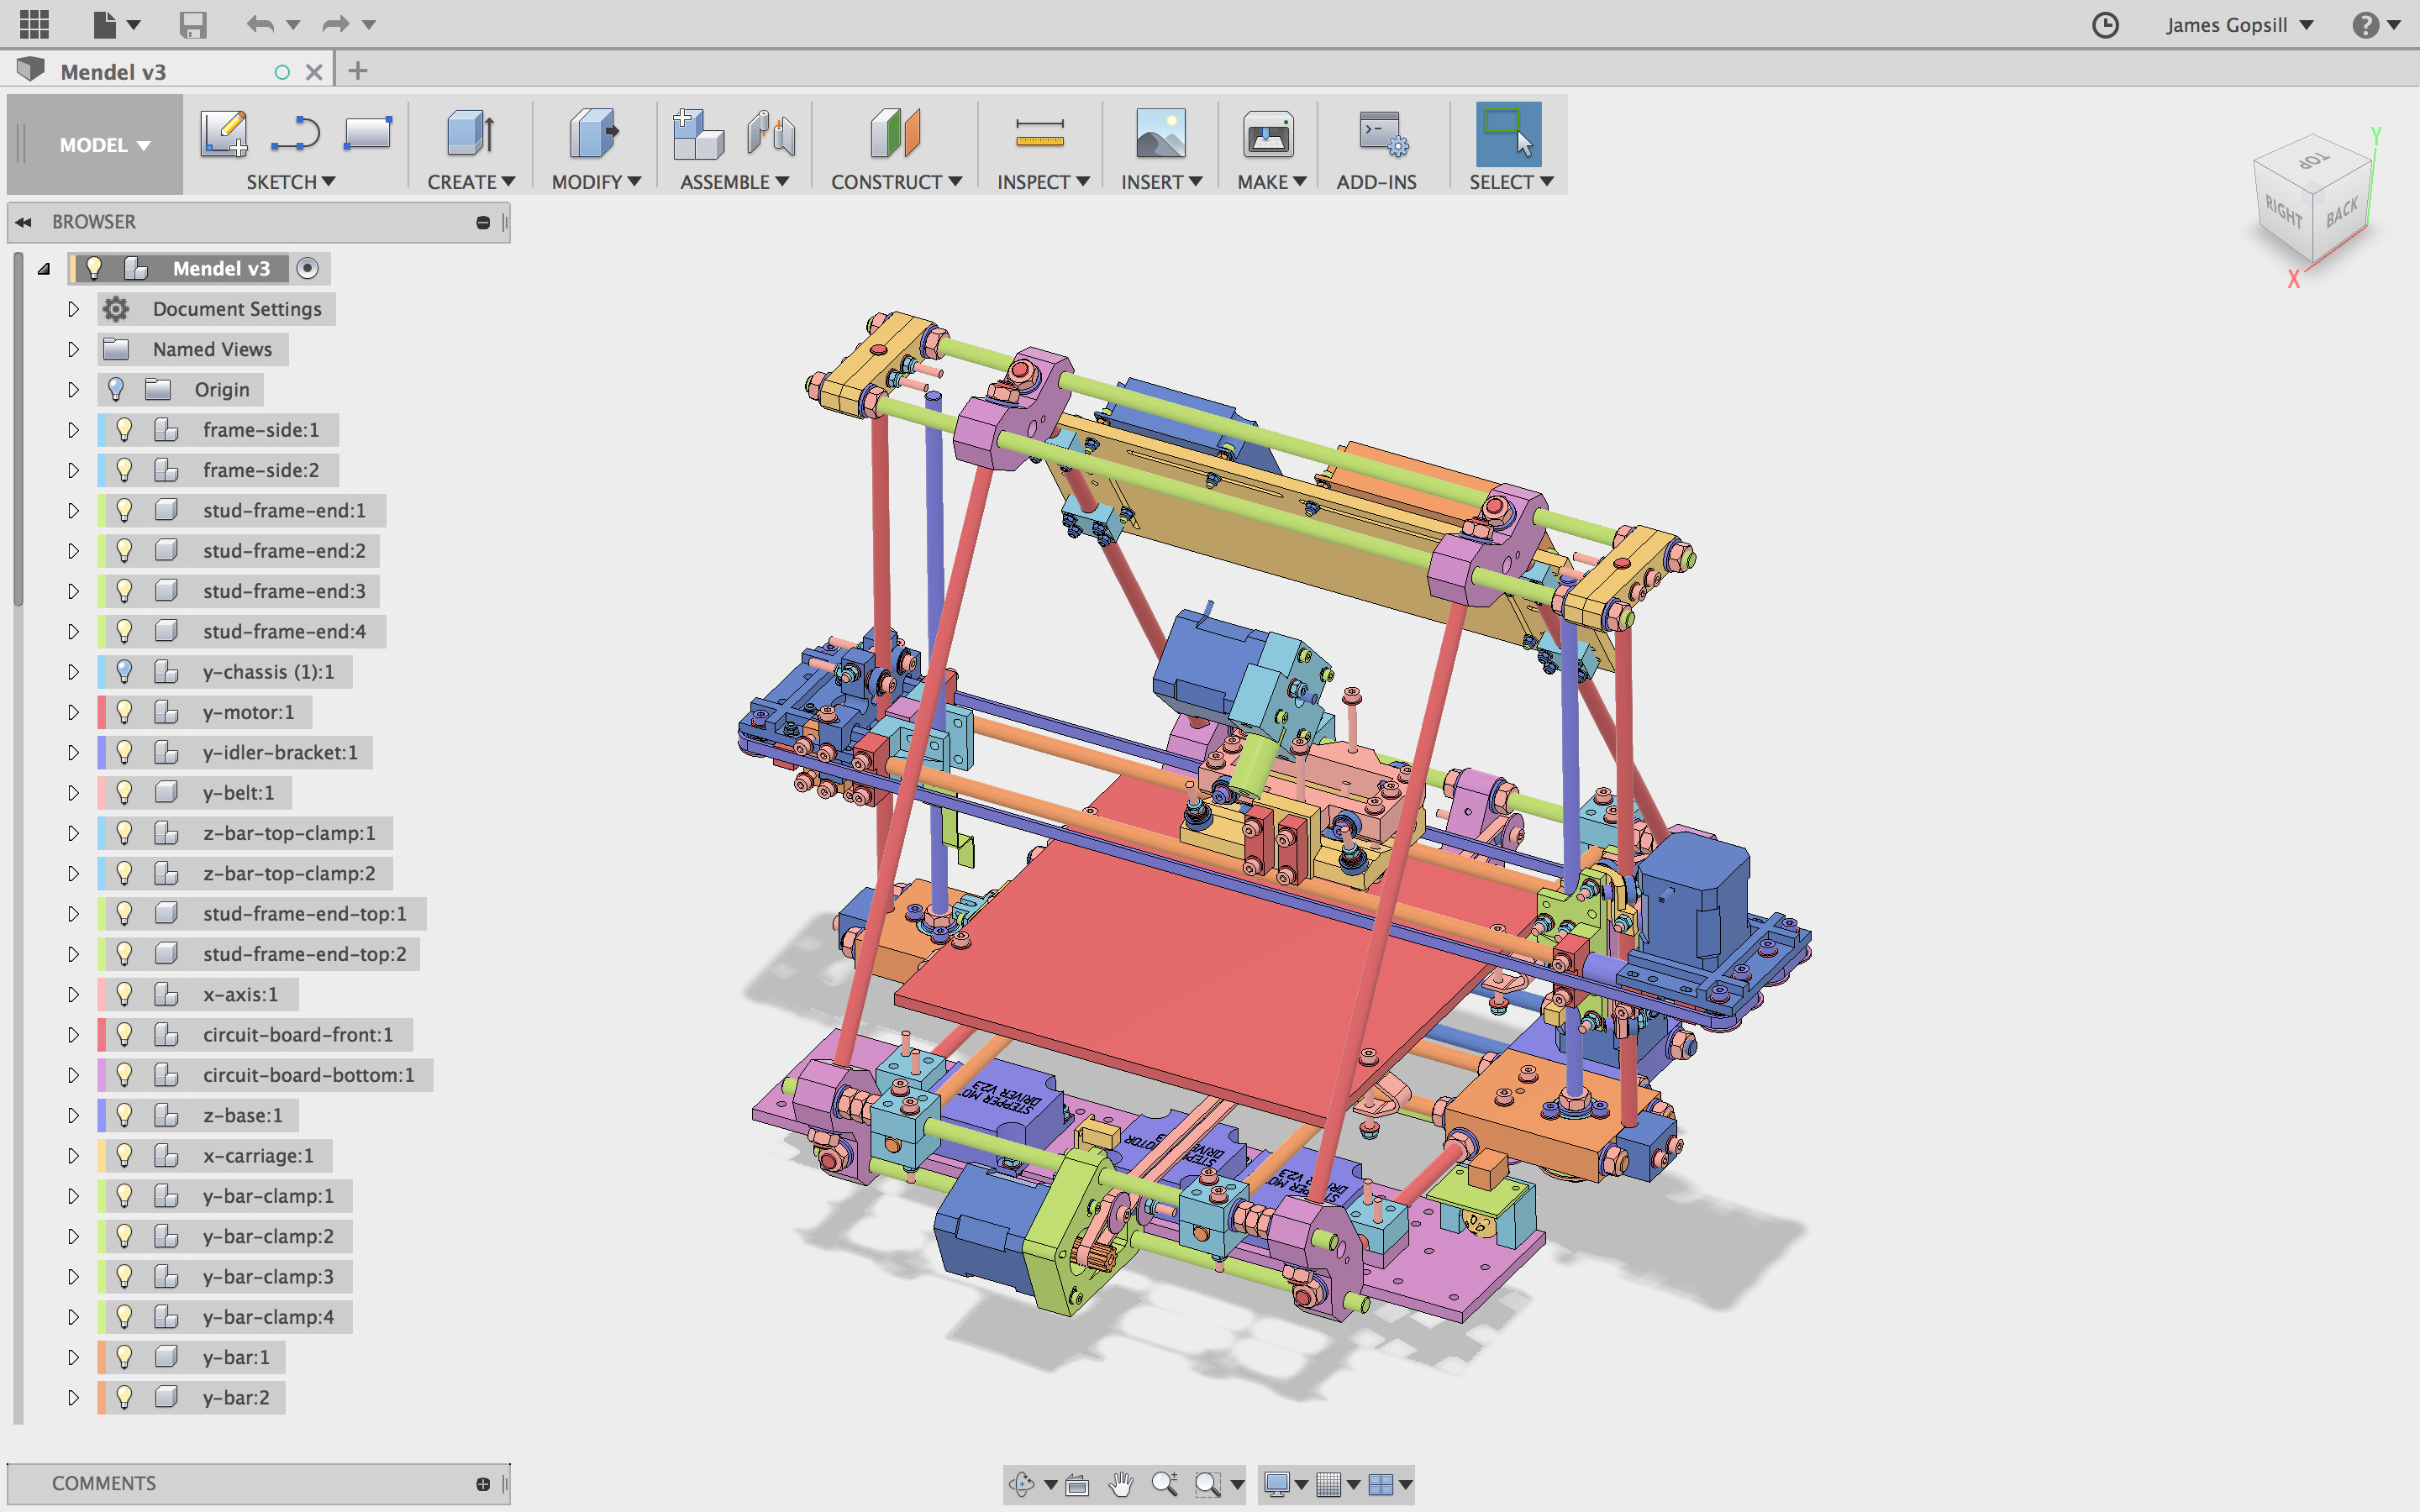
\includegraphics[width=0.4\textwidth]{figures/Mendel-2.png}
    \end{tikzfigure}
  }
  \block[]{Infill Optimisation}{
    \textbf{Using Finite Element Analysis to Influence the Infill Design of Fused Deposition Modelled Parts}\\
    \small
    J.A. Gopsill, J. Shindler \& B.J. Hicks\\
    Progress in Additive Manufacturing
    \begin{tikzfigure}[Infill generation process]
      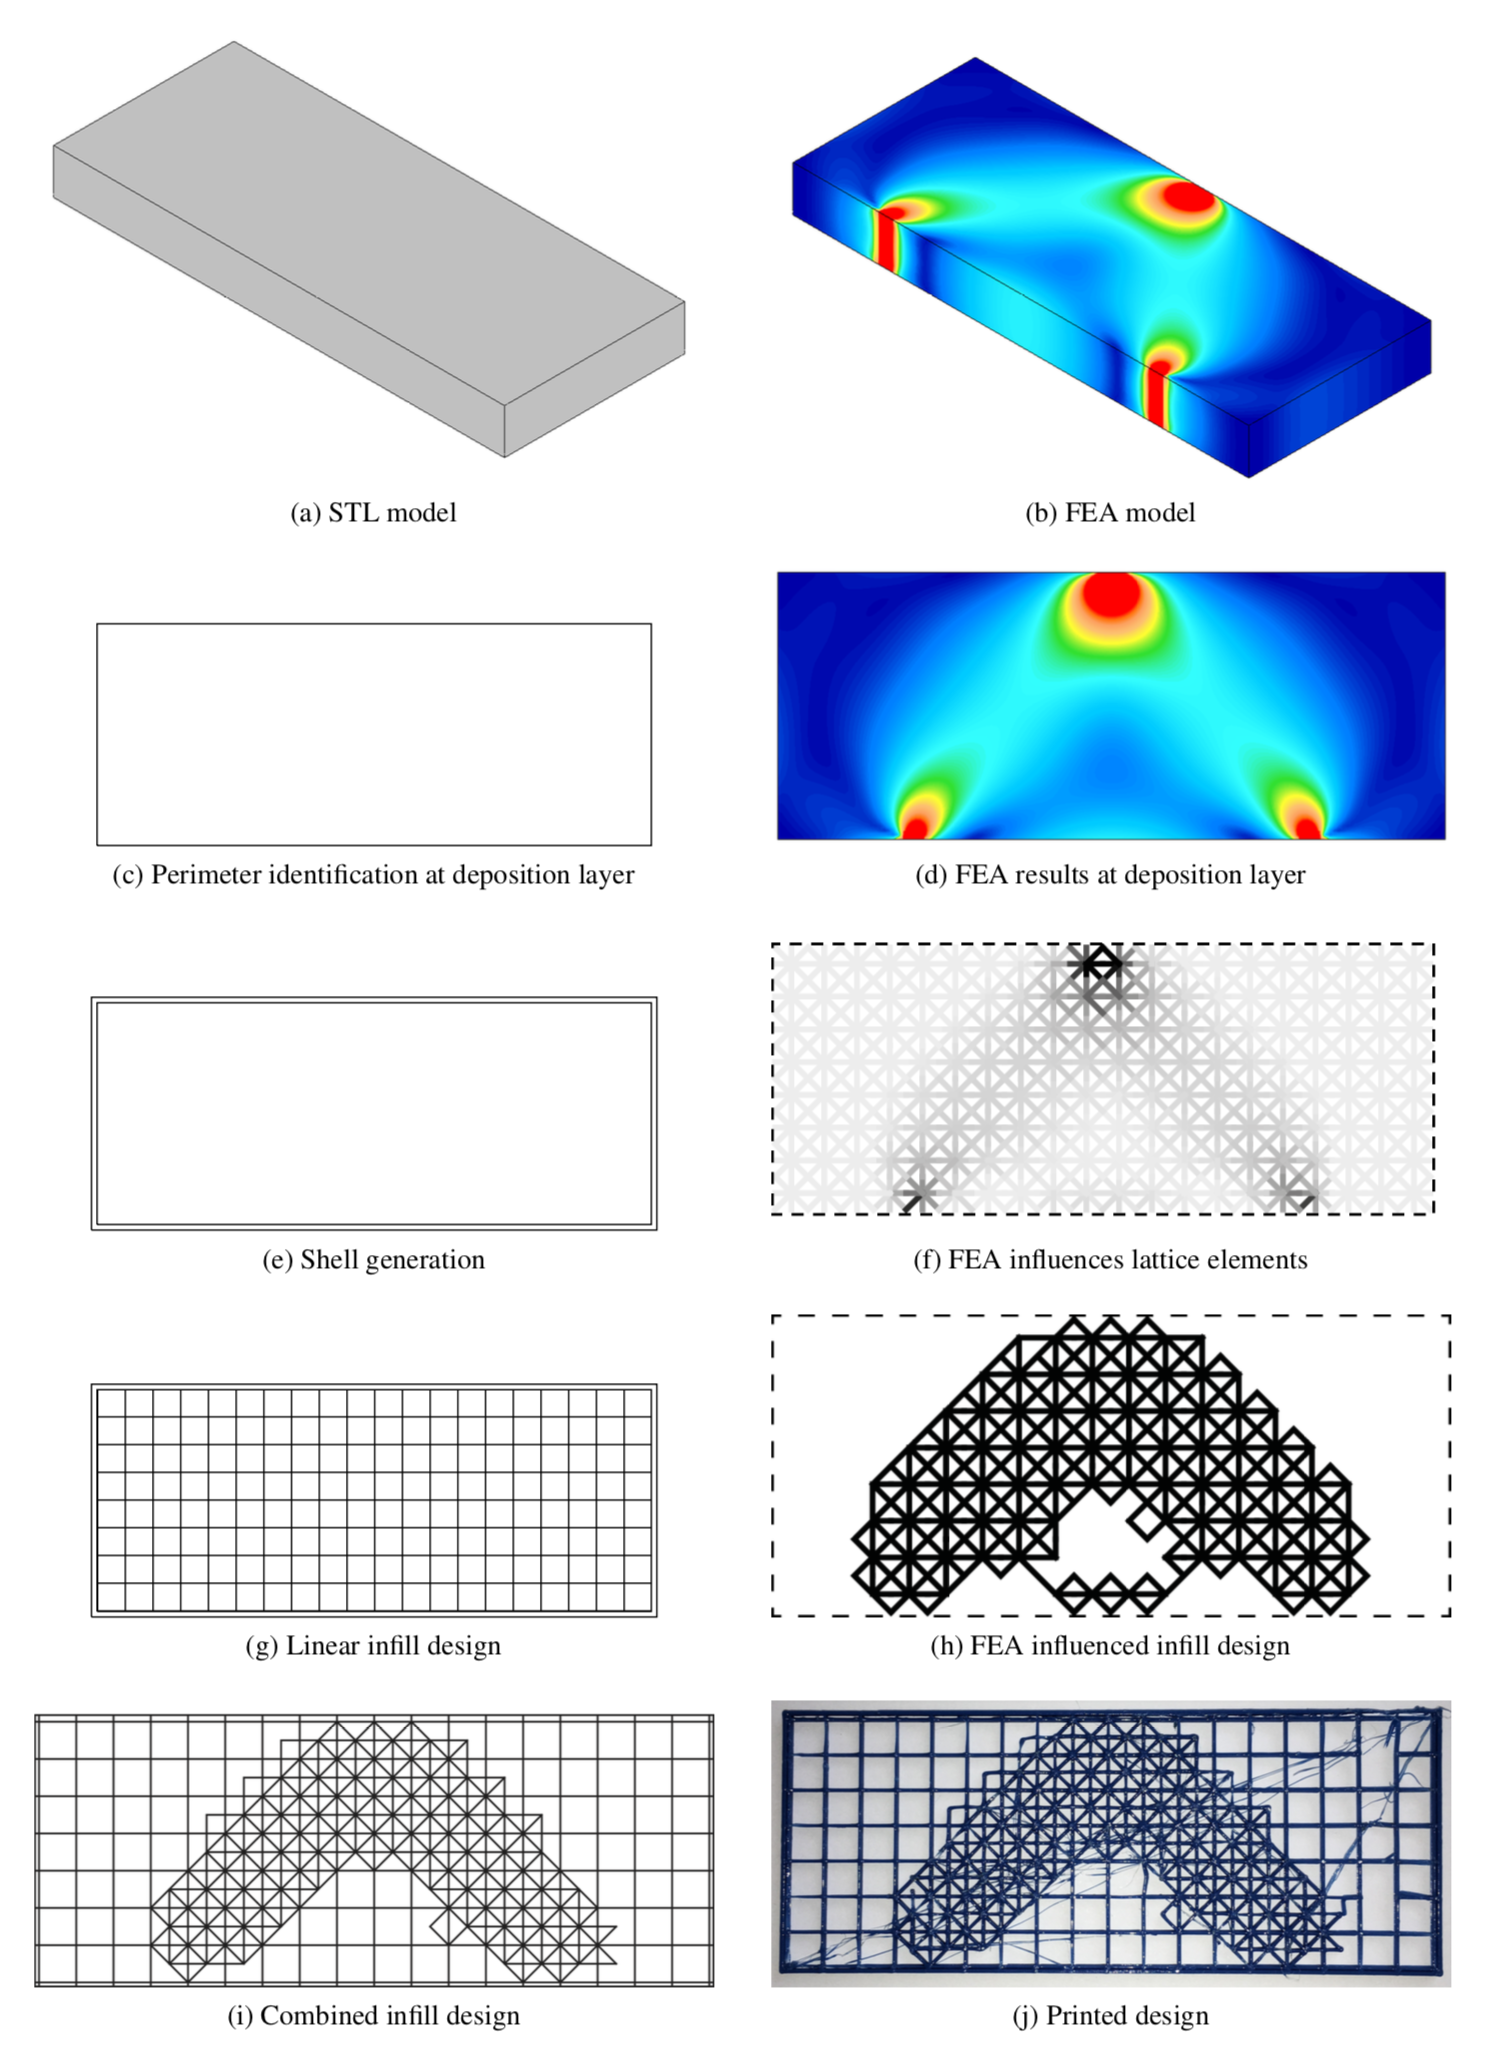
\includegraphics[width=0.3\textwidth]{figures/optimisation.png}
    \end{tikzfigure}
  }
  \block[]{Project Management Support}{
    \textbf{A Sequence-based Approach to Analysing and Representing Engineering Project Normality} \\
    \small
    L. Shi, J.A. Gopsill, L. Newnes, S.J. Culley\\
    IEEE International Conference on Tools with Artificial Intelligence
    \begin{tikzfigure}[Workload modelling of aircraft maintenance events]
      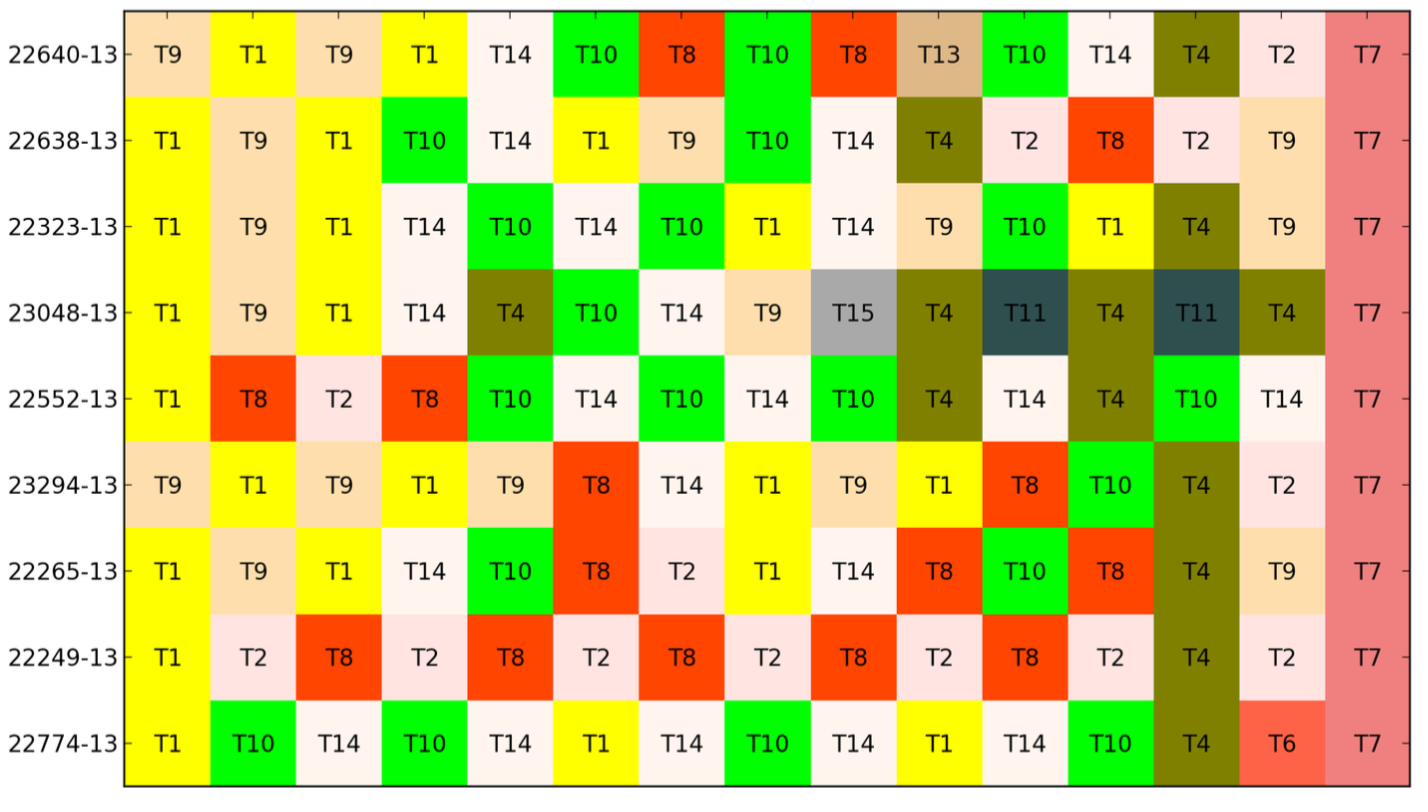
\includegraphics[width=0.2\textwidth]{figures/sequence.png}
    \end{tikzfigure}
  }
  \column{0.5}
  \block[]{Meaning from Metadata}{
    \textbf{Automatic generation of design structure matrices through the evolution of product models}\\
    \small
    J.A. Gopsill, C. Snider, C. McMahon \& B.J. Hicks\\
    Artificial Intelligence for Engineering Design, Analysis and Manufacturing
    \begin{tikzfigure}[Modelling system architectures through metadata]
      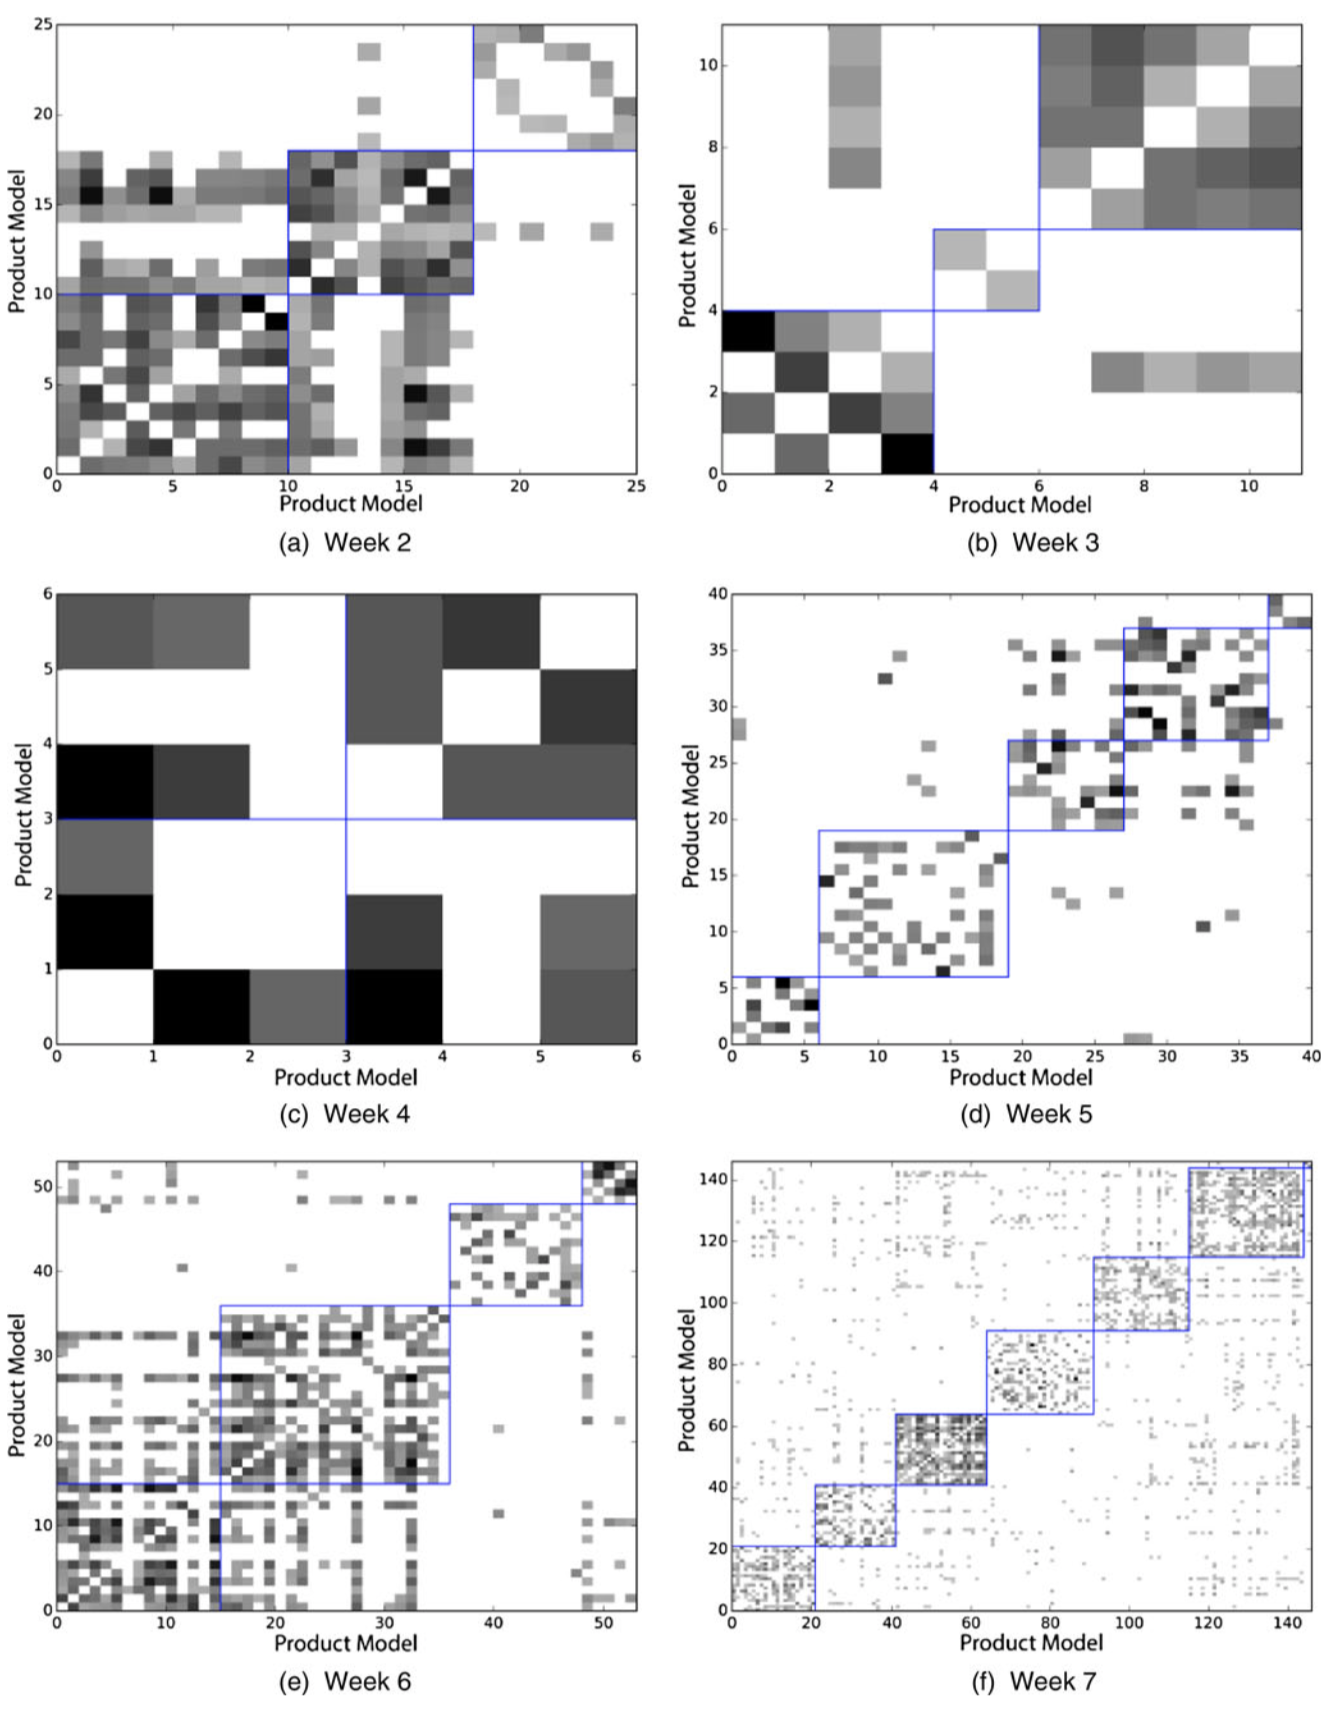
\includegraphics[width=0.25\textwidth]{figures/dsm.png}
    \end{tikzfigure}
  }
  \block[]{Principles of Construction Kits}{
    \textbf{Examining the Solution Bias of Construction Kits}\\
    \small
    J.A. Gopsill\\
    International Conference on DESIGN
    \begin{tikzfigure}[Analysing the combinatorics of construction kits]
      \small
      \begin{tabular}{c c}
        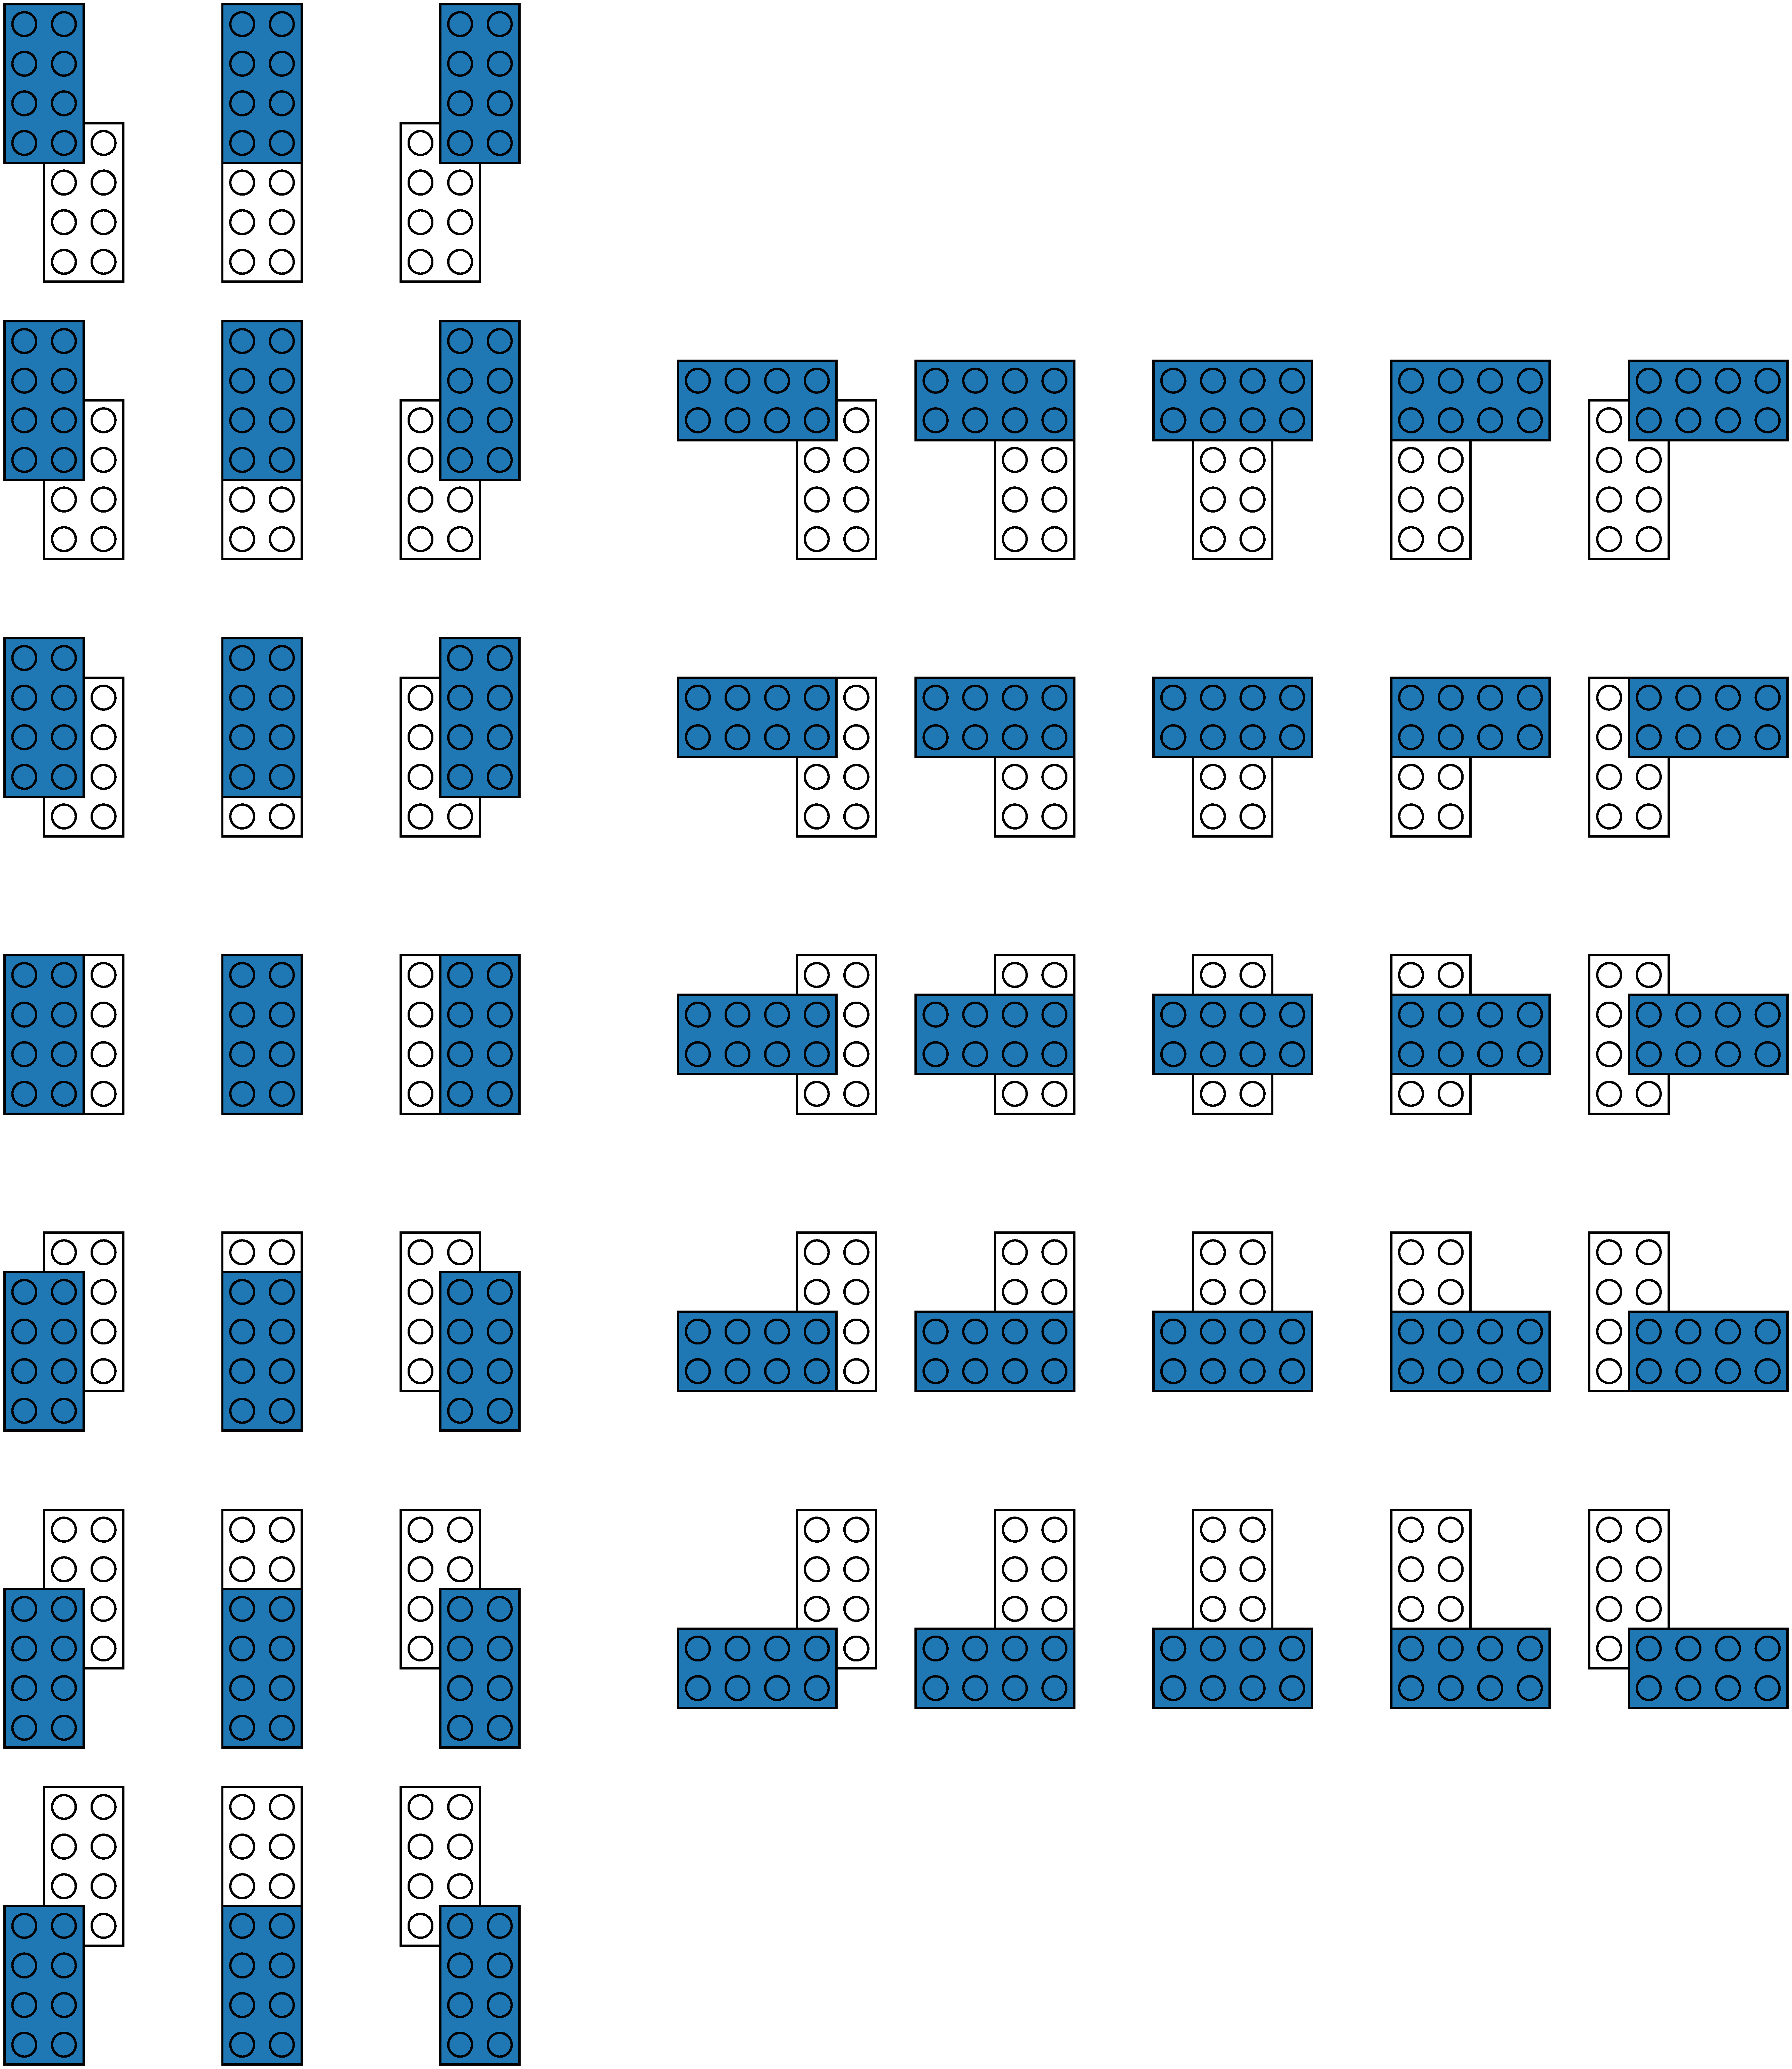
\includegraphics[width=0.2\textwidth]{figures/2-2x4-combinations.pdf}
        &
        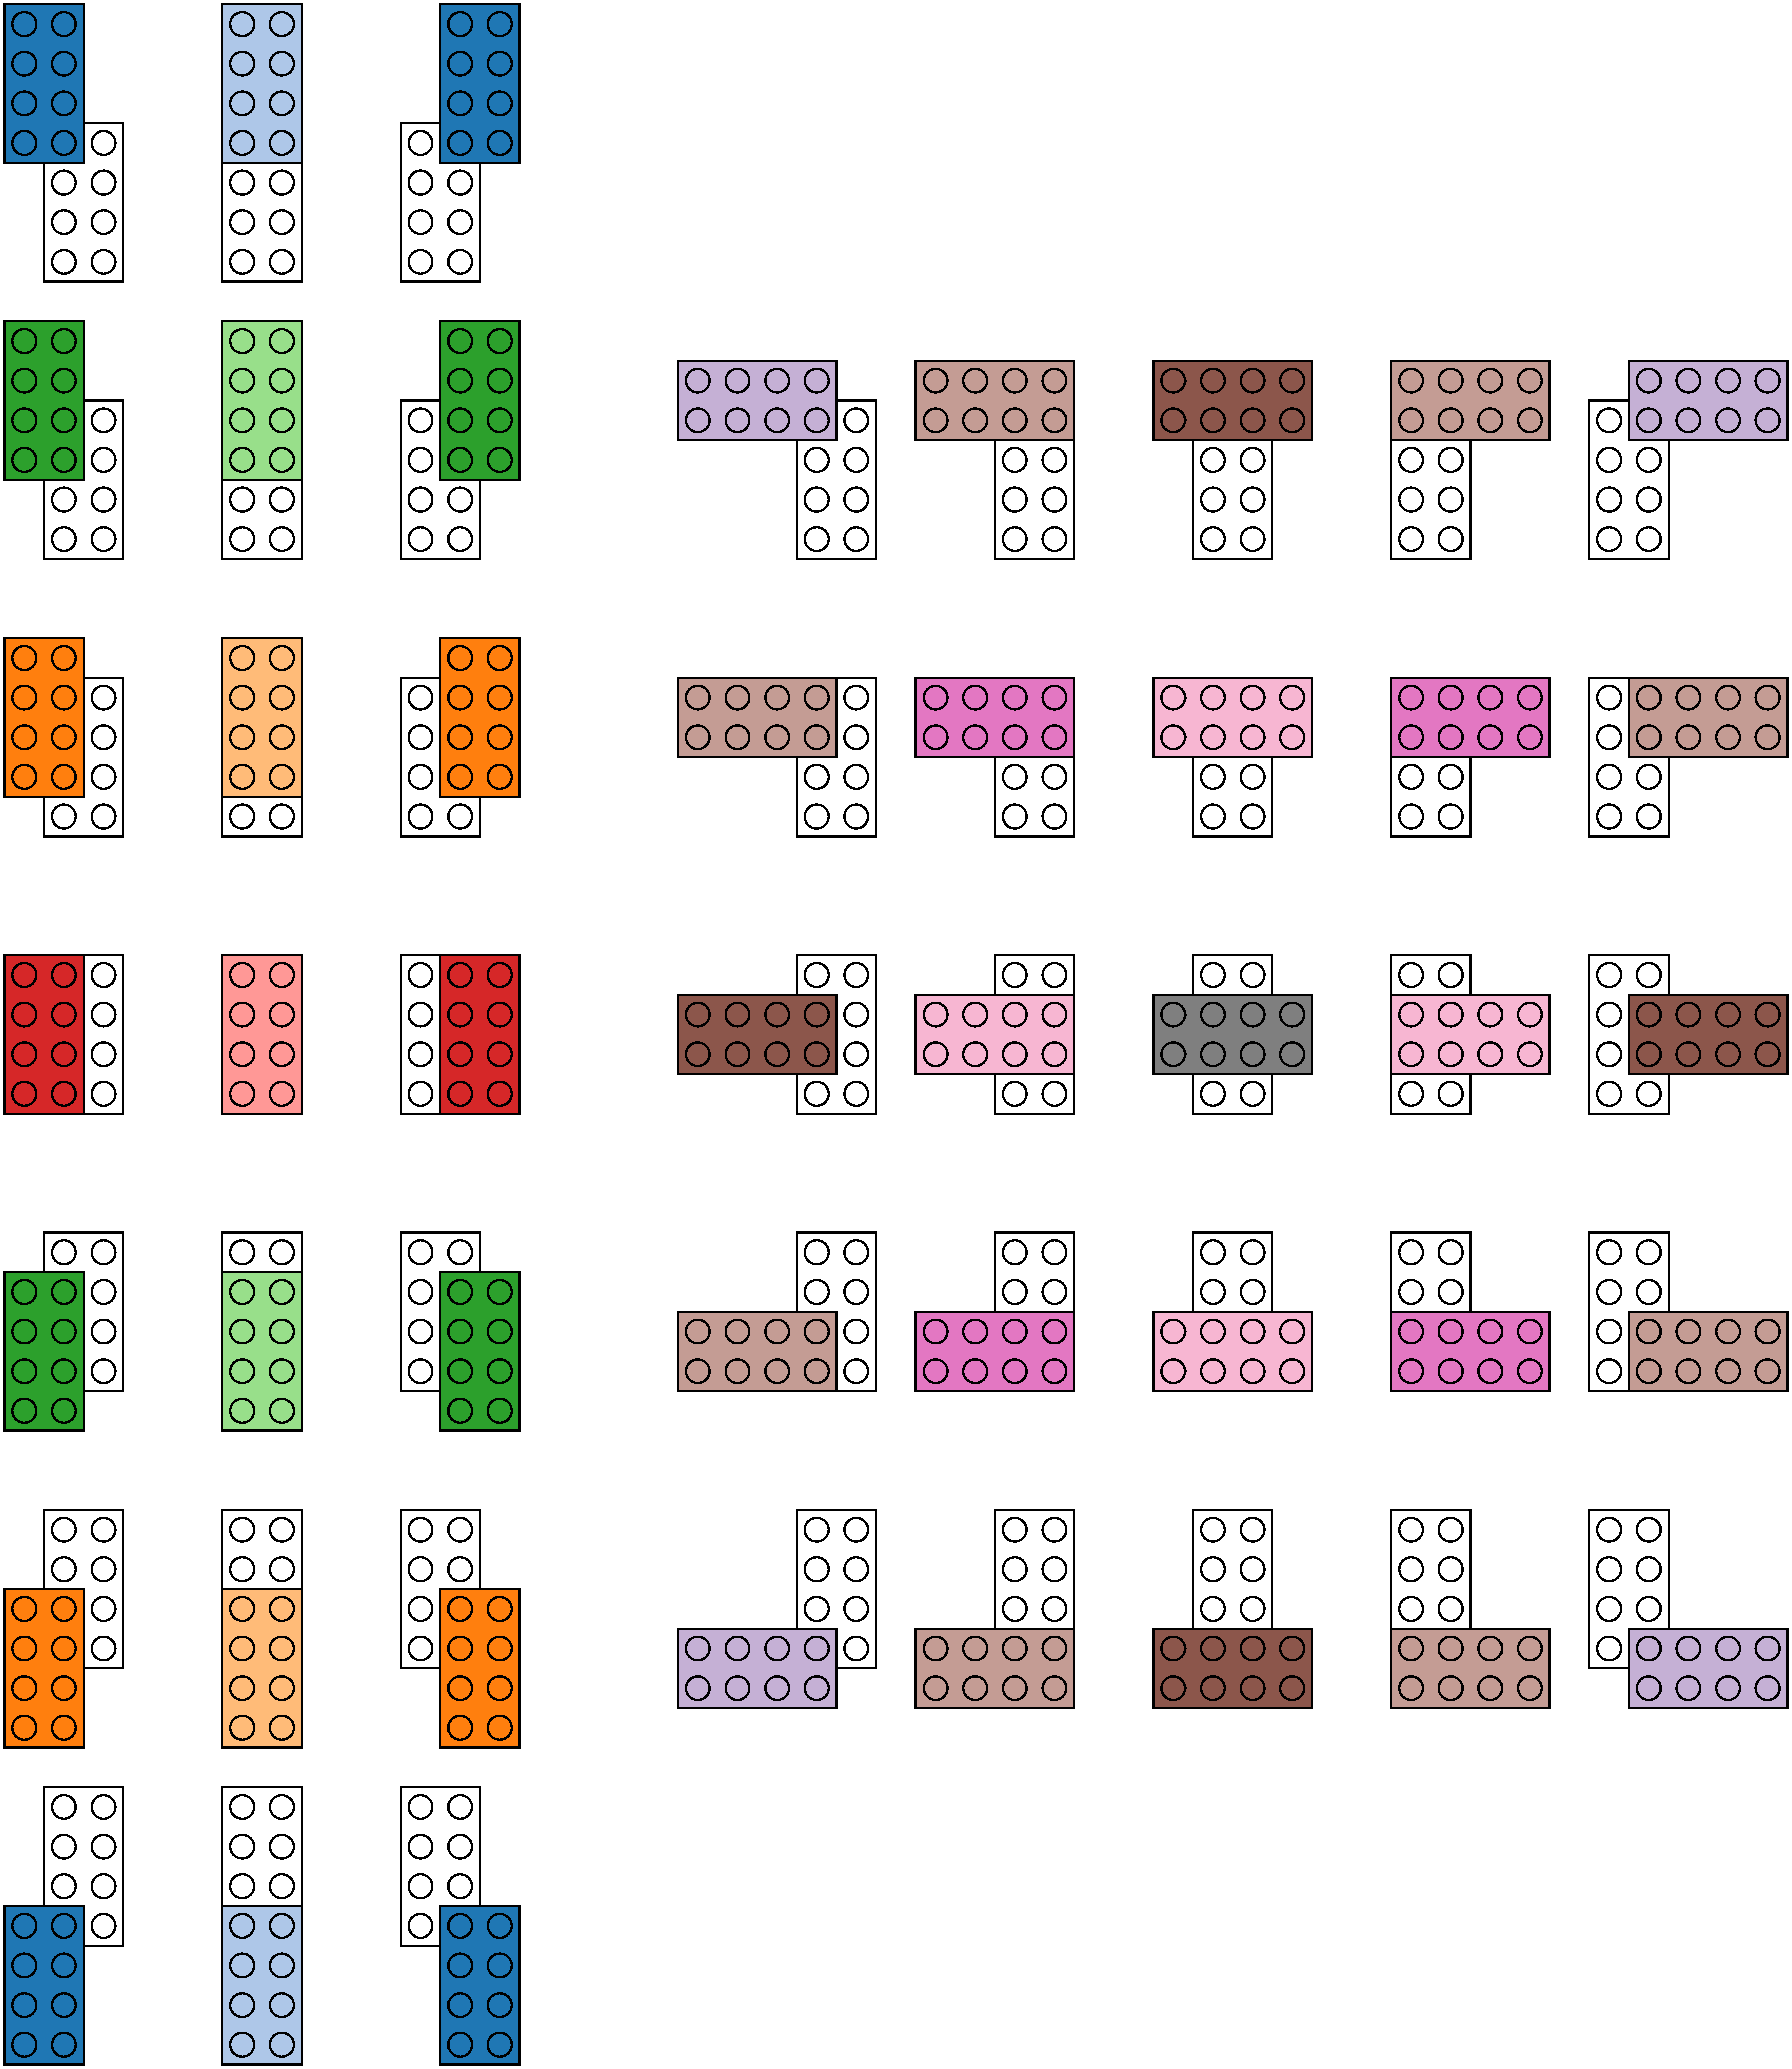
\includegraphics[width=0.2\textwidth]{figures/2-2x4-combinations-colored.pdf}
        \\

        The 46 combinations of $B_{2,4}(2)$
        &
        14 \textbf{morphologically} unique combinations of $B_{2,4}(2)$ \\
        \\
        \multicolumn{2}{c}{
          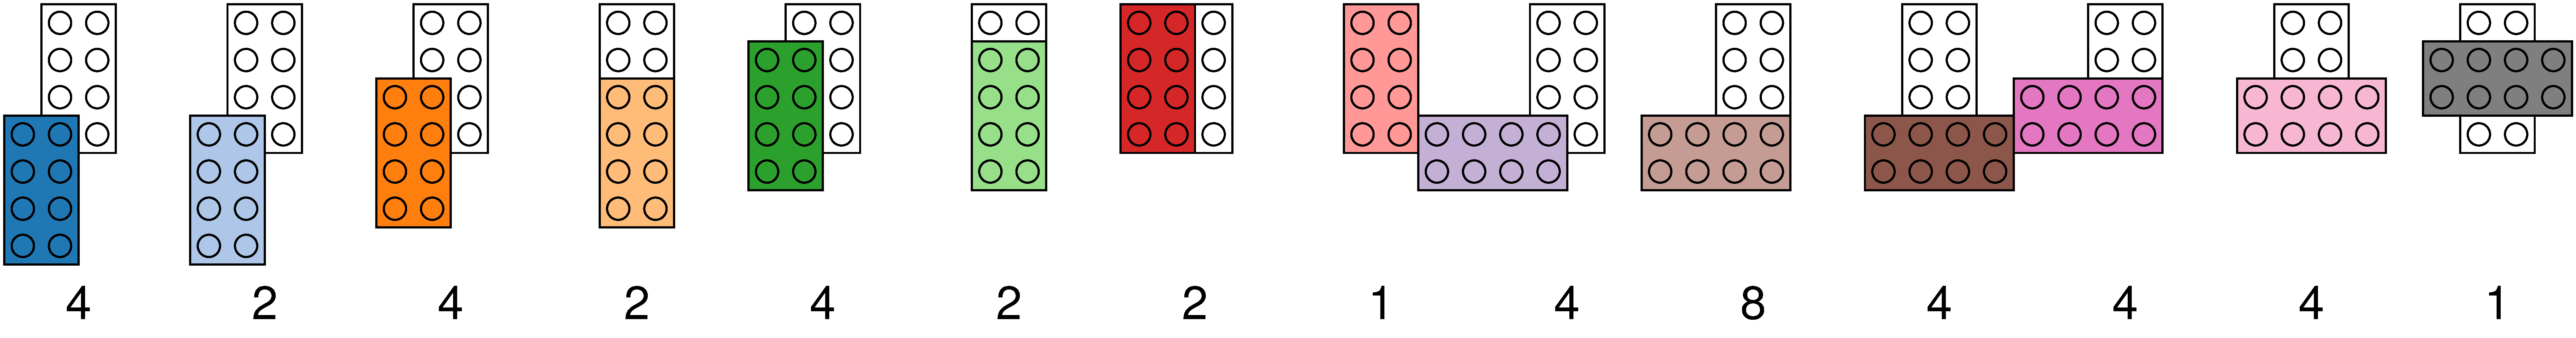
\includegraphics[width=0.4\textwidth]{figures/combinations.pdf}
        } \\
        \multicolumn{2}{c}{
          Number of pathways to each morphologically unique combination
        } \\
      \end{tabular}
    \end{tikzfigure}
  }

  \block[]{Competency Mapping}{
    \textbf{RCUK Researcher in Residence at the National Composites Centre}\\
    \small
    J.A. Gopsill
    \begin{tikzfigure}[Automatic generation of competency maps through design report analysis]
      \begin{tabular}{c c}
        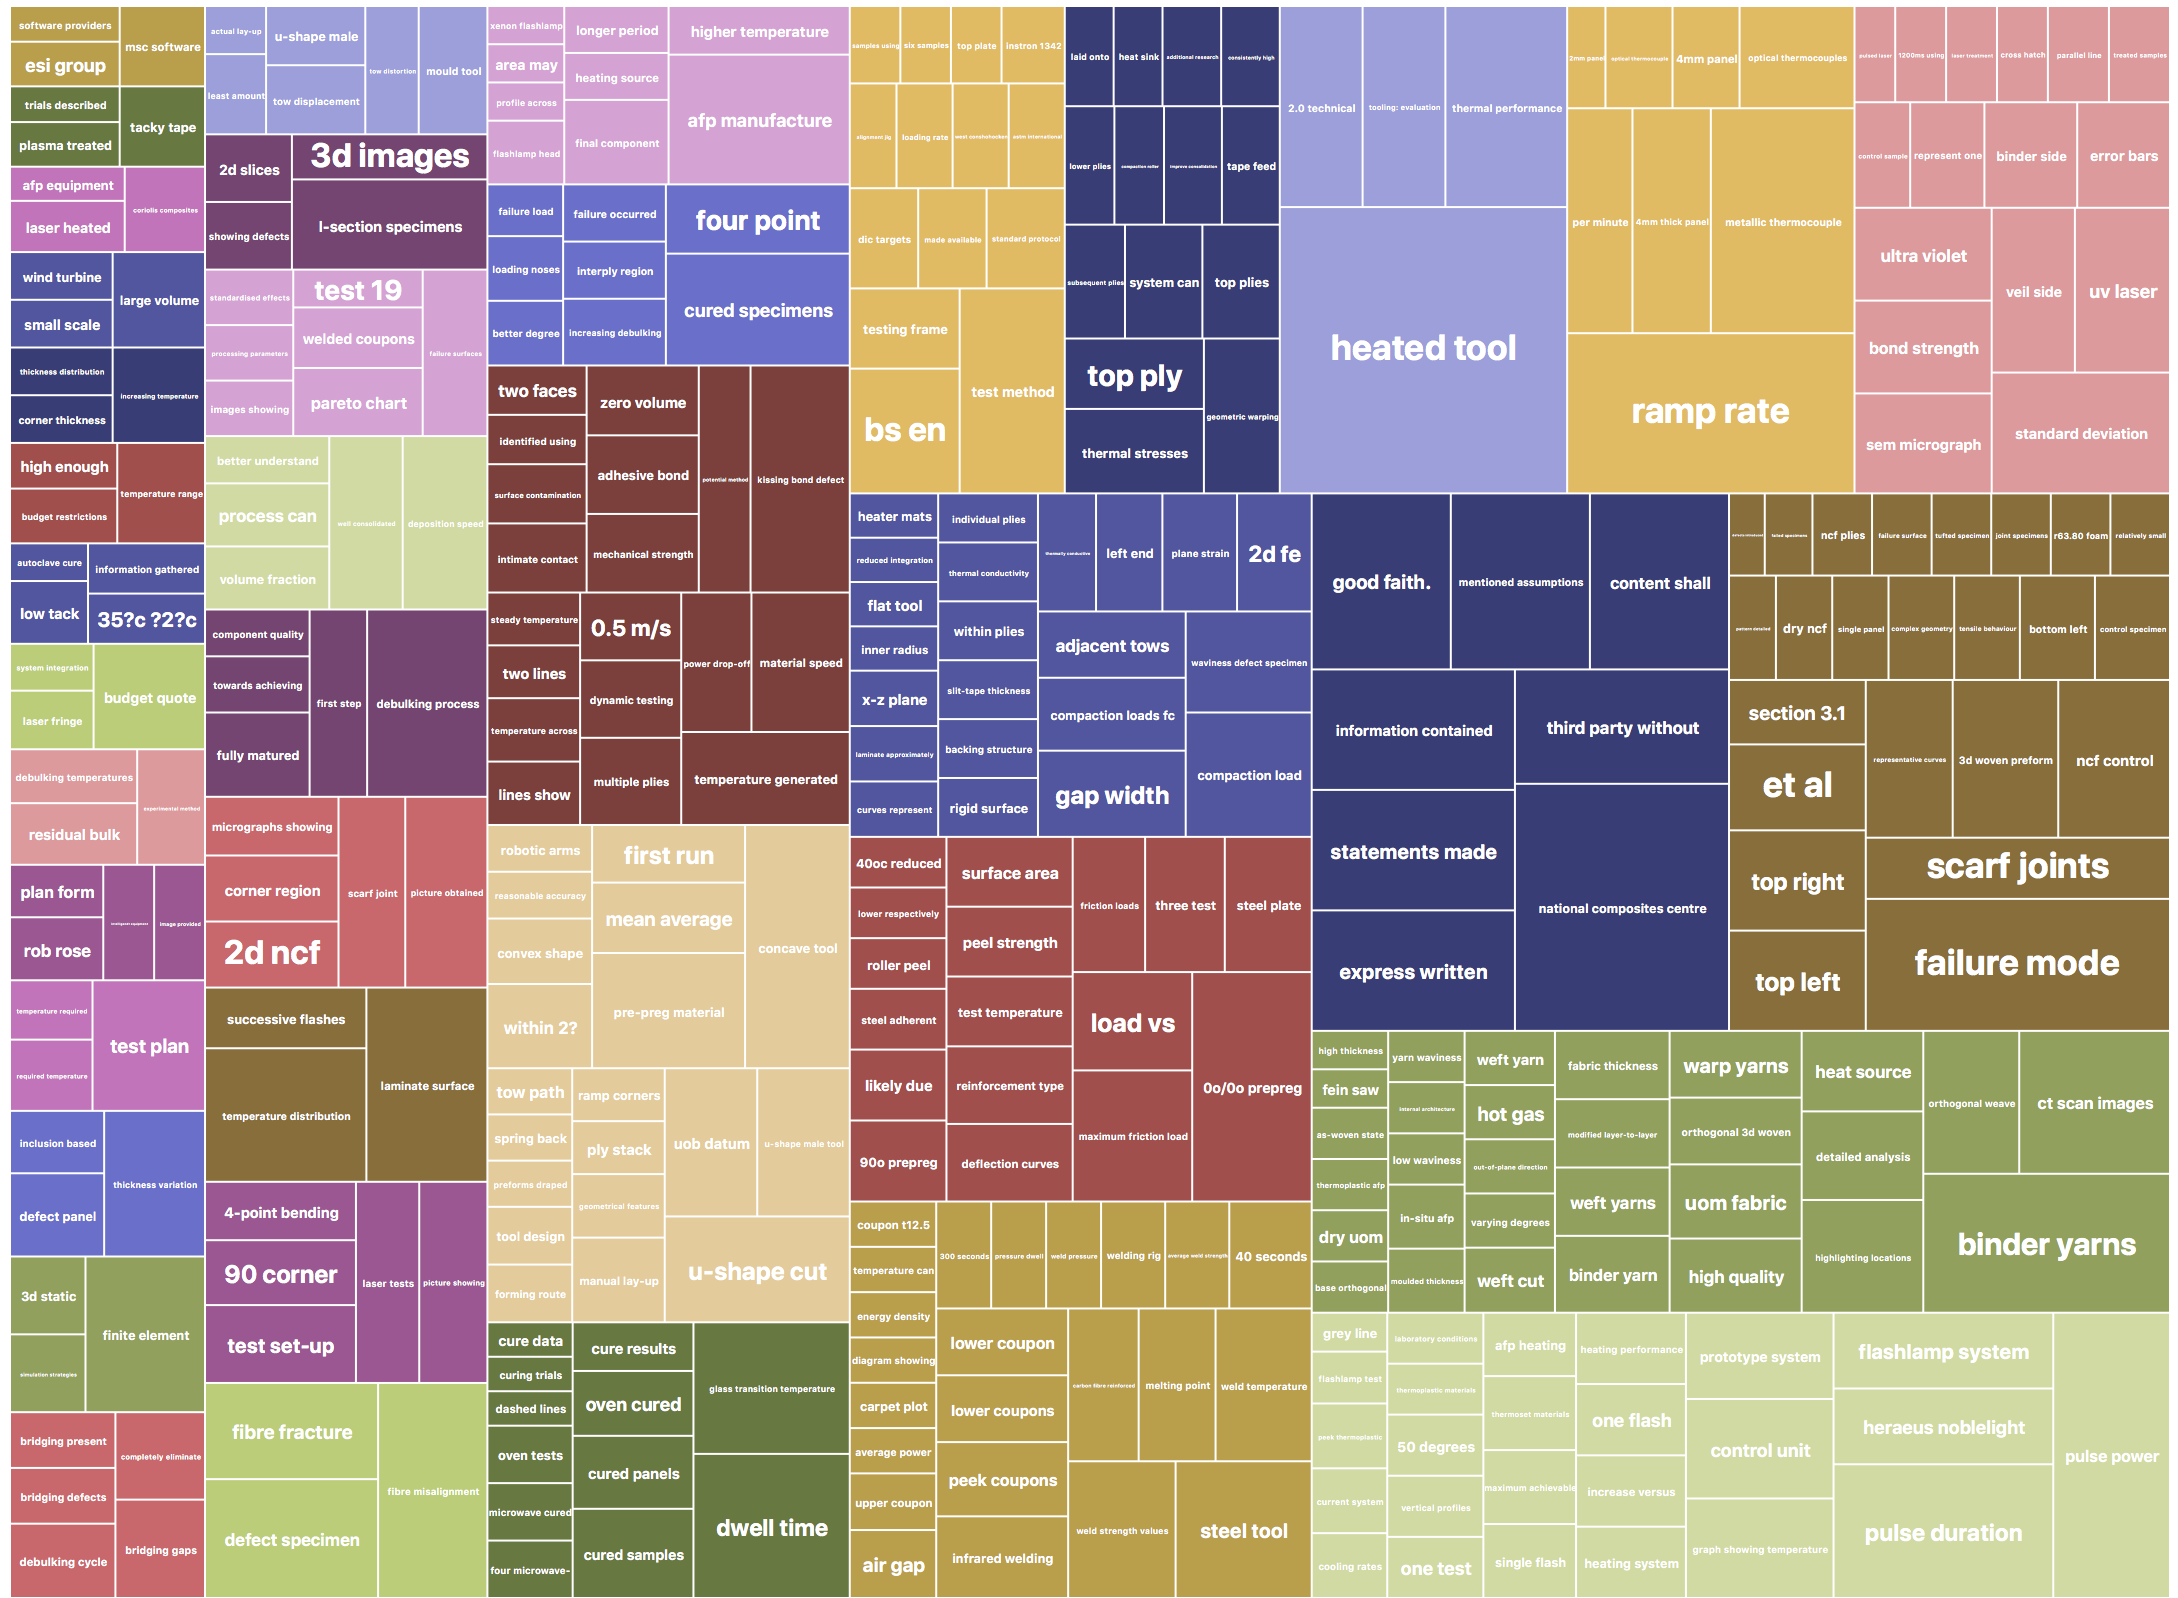
\includegraphics[width=0.2\textwidth]{figures/competencies.png} &
        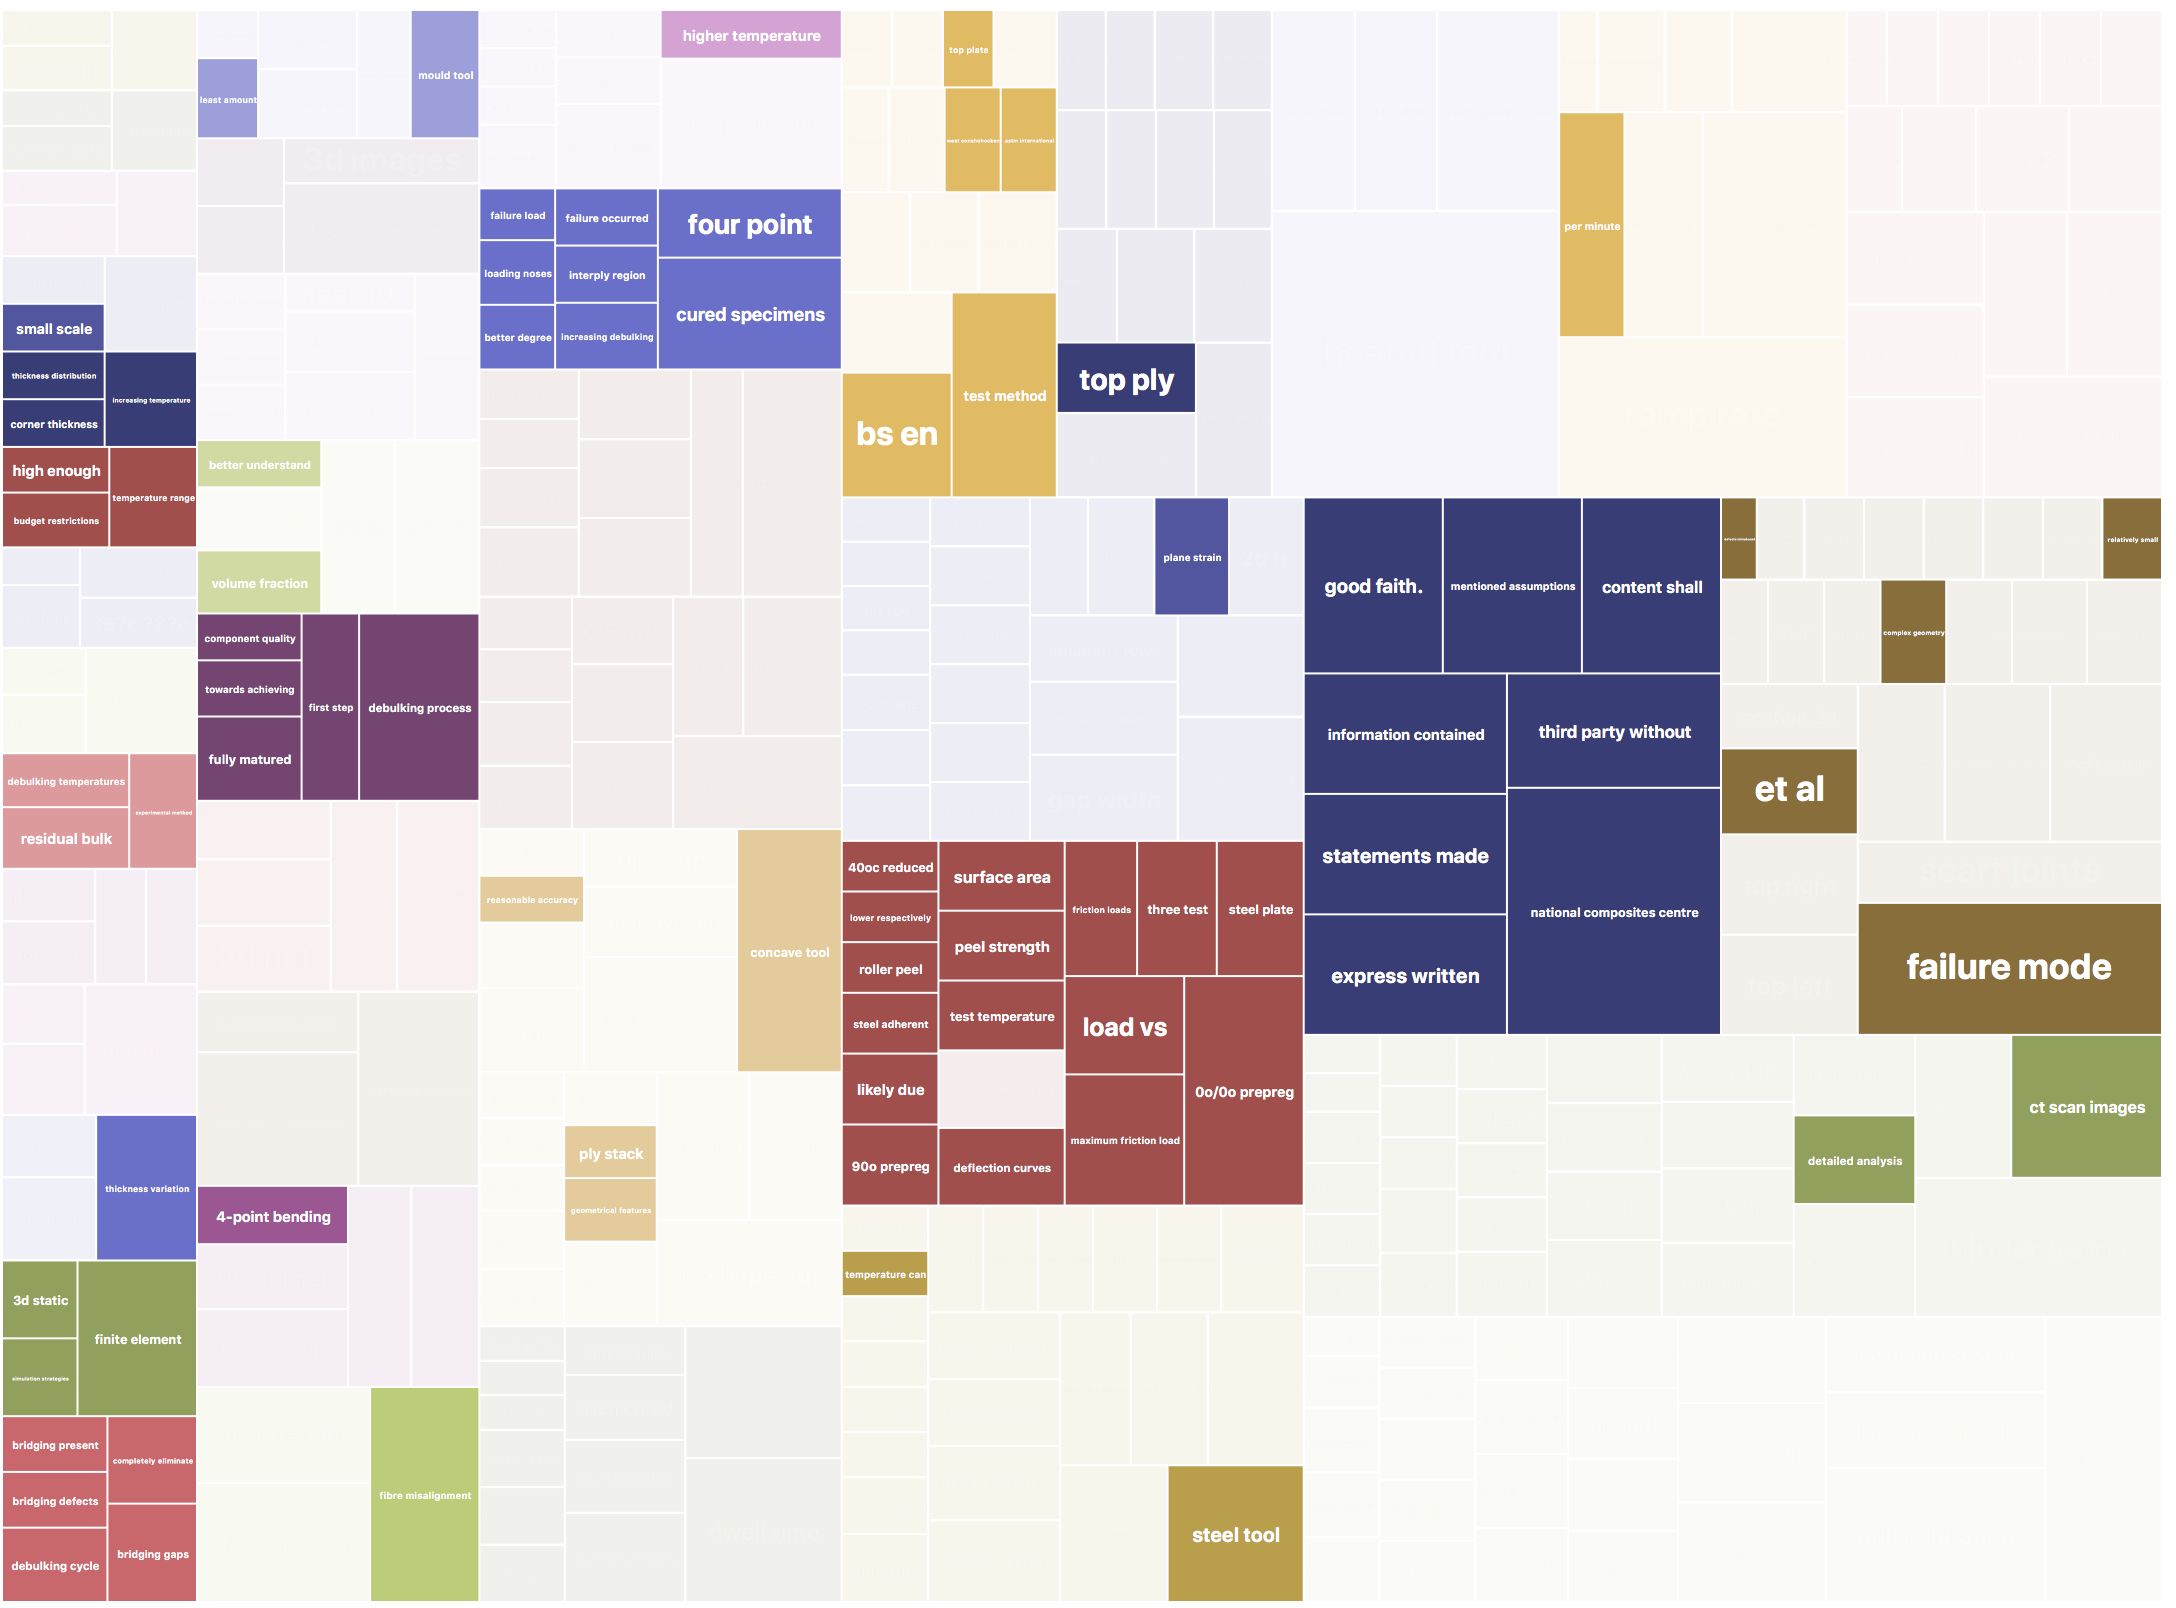
\includegraphics[width=0.2\textwidth]{figures/person.png} \\
        Organisation Competency Map &
        Expert Competency Map \\
      \end{tabular}
    \end{tikzfigure}
  }
\end{columns}


\end{document}